\RequirePackage{luatex85}
\documentclass[border={20pt,20pt,20pt,20pt}]{standalone}

\usepackage[dvipsnames]{xcolor}
\usepackage{tikz}
\usetikzlibrary{shapes, patterns, calc}

\begin{document}
	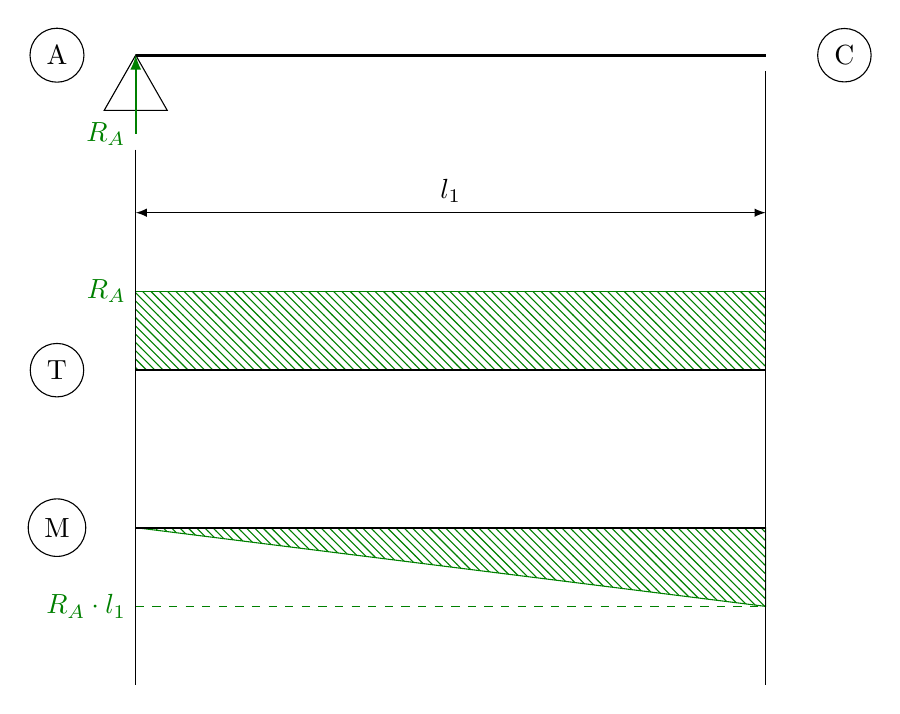
\begin{tikzpicture}[
	label/.style={circle,draw},
	gFill/.style={Green, pattern=north west lines, pattern color=Green},
	arrow/.style={latex-latex}
	]
	
	\coordinate (A) at (0, 0);
	\coordinate (C) at (8, 0);
	
	\draw[very thick] (A) -- (C);
	\node [label] at ($(A) + (-1,0)$) {A};
	\node [label] at ($(C) + (1, 0)$) {C};
	
	\draw [arrow] ($(A) - (0, 2)$) -- ($(C) - (0, 2)$) node[midway, above] {$l_1$};
	
	\draw (A) -- ($(A) - (.4,.7)$) -- ($(A) + (+.4, -.7)$) -- cycle;
	
	\coordinate (N1) at ($(A)$);
	\coordinate (N2) at ($(C)$);
	\coordinate (T1) at ($(N1) - (0, 4)$);
	\coordinate (T2) at ($(N2) - (0, 4)$);
	\coordinate (M1) at ($(T1) - (0, 2)$);
	\coordinate (M2) at ($(T2) - (0, 2)$);
	
	% Tallant
	\node [label] at ($(T1) - (1, 0)$) {T};
	\draw[gFill] (T1) rectangle ($(T2) + (0, 1)$);
	\draw[thick] (T1) -- (T2);
	\node[Green, anchor=east] at ($(T1) + (0, 1)$) {$R_A$};
	
	% Moment
	\node [label] at ($(M1) - (1, 0)$) {M};
	\draw[gFill] (M1) -- ($(M2) - (0, 1)$) -- (M2) -- cycle;
	\draw[thick] (M1) -- (M2);
	\draw[Green, dashed] ($(M1) - (0, 1)$) -- ($(M2) - (0, 1)$);
	\node[Green, anchor=east] at ($(M1) - (0, 1)$) {$R_A \cdot l_1$};
	
	\draw ($(A) - (0, 1.2)$) -- ($(M1) - (0, 2)$);
	\draw ($(C) - (0, .2)$) -- ($(M2) - (0, 2)$);
	
	\draw[Green, thick,-latex] ($(A) - (0, 1)$) -- (A) node [at start, left] {$R_A$};
	\end{tikzpicture}
\end{document}